%
% hardware.tex
%
% Copyright The TTC 2.0 Contributors.
%
% TTC 2.0 Documentation
%
% This work is licensed under the Creative Commons Attribution-ShareAlike 4.0
% International License. To view a copy of this license,
% visit http://creativecommons.org/licenses/by-sa/4.0/.
%

%
% \brief Hardware project chapter.
%
% \author Gabriel Mariano Marcelino <gabriel.mm8@gmail.com>
%
% \version 0.3.0
%
% \date 2021/04/02
%


\chapter{Hardware} \label{ch:hardware}

This chapter presents a description about the hardware project of the TTC 2.0 moduel. As a main reference, a block diagram can be seen in \autoref{fig:hardware-diagram}.

\begin{figure}[!h]
	\begin{center}
		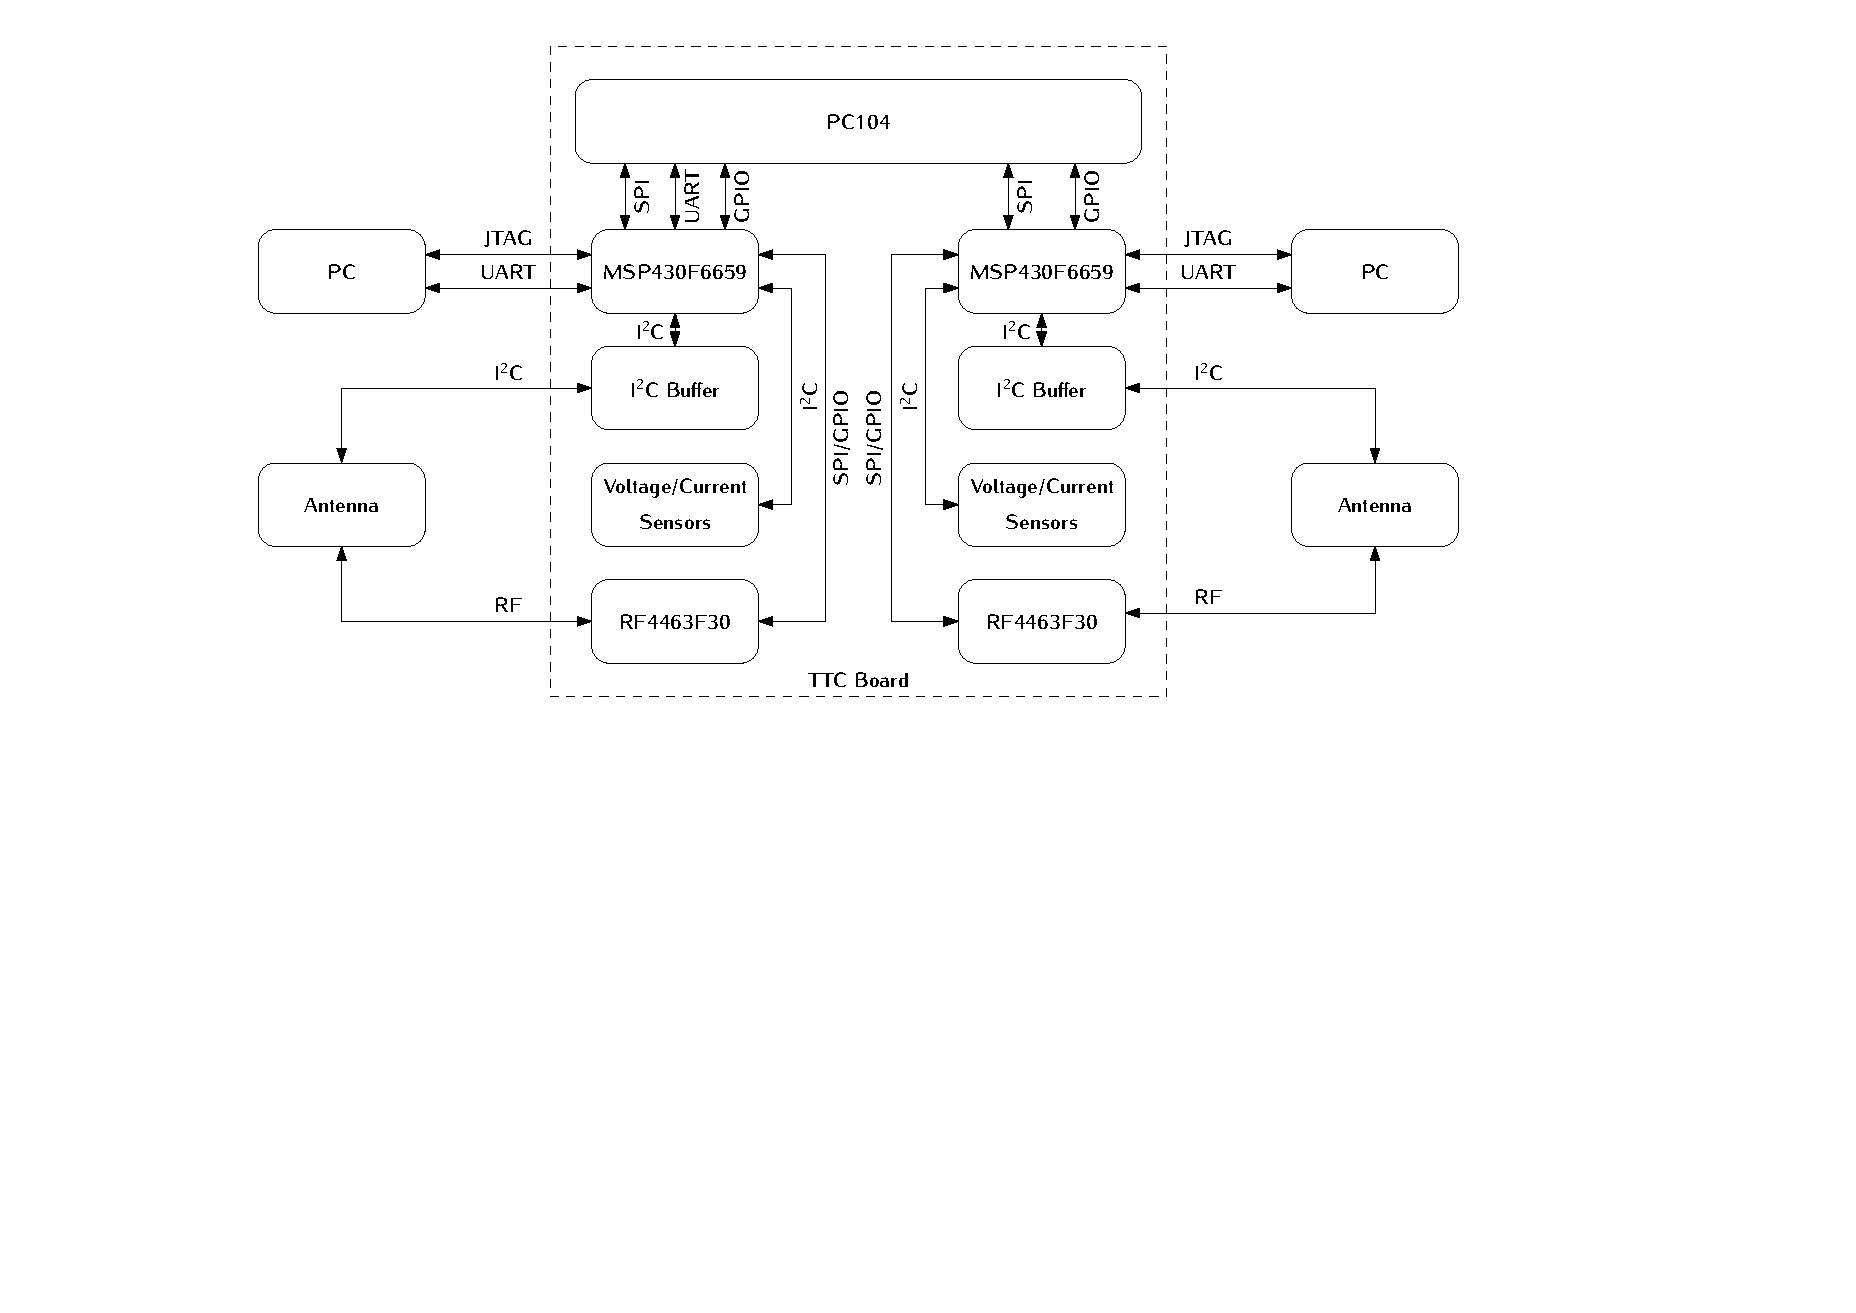
\includegraphics[width=\textwidth]{figures/hardware_diagram.pdf}
		\caption{Block diagram of the TTC 2 hardware.}
		\label{fig:hardware-diagram}
	\end{center}
\end{figure}

In the next sections, a further description of the hardware project is presented.

\section{Specifications}

The TTC 2.0 has two microcontrollers (MSP430FR6659) that runs at a clock of 32 MHz, a RAM memory of 64 kB (SRAM), and a flash memory of 512 kB for code storage, and another one of 128 kB for data storage. The TTC 2.0 also has current, voltage and temperature sensors, and two radio modules for RF communication. A brief description of the general specifications of the TTC 2.0 module is available below:

\begin{itemize}
    \item \textbf{Microcontroller}: MSP430F6659
    \item \textbf{Clock}: 32 MHz
    \item \textbf{Memories}:
    \begin{itemize}
        \item RAM: 64 kB (SRAM)
        \item Flash: 512 kB (code)
    \end{itemize}
    \item \textbf{Sensors}: Voltage, current and temperature
    \item \textbf{Modulation}: (G)FSK and (G)MSK
    \item \textbf{Baudrate}: 1200 to 9600 bps
    \item \textbf{Frequency}: 145-146 MHz, 435-438 MHz and 450 MHz bands
    \item \textbf{Protocol}: NGHam
    \item \textbf{Interfaces}: UART, I$^{2}$C and SPI
    \item \textbf{Mass}: 73 g
    \item \textbf{Main bus}: PC-104 standard
\end{itemize}

\subsection{RF Communication}

The module can operate using the following modulations: FSK, MSK GFSK or GMSK. The baudrate can be between 1200 bps to 9600 bps. The TTC 2.0 uses ISIS antenna with UHF and VHF in mode.... ( mais detalhes) operating in the 145-146 MHz and 435-438 MHz or 450 Mhz bands.

\section{PC-104 Bus}

The connector referred as PC-104 is a junction of two double row 26 pin headers (\textit{SSW-126-04-G-D}). These connectors create a solid 104-pin interconnection across the different satellite modules. \autoref{tab:pc104-pinout} provides the connector pinout\footnote{This pinout is simplified since additional interfaces were omitted. Refer to \textit{option sheet} in chapter \ref{ch:assembly}.} for the pins that are connected to the module. A reference of the pins' position can also be seen in \autoref{fig:pc104-ref-diagram}, a description of the signal is available in \autoref{tab:pc104-signals}.

\begin{figure}[!ht]
    \begin{center}
        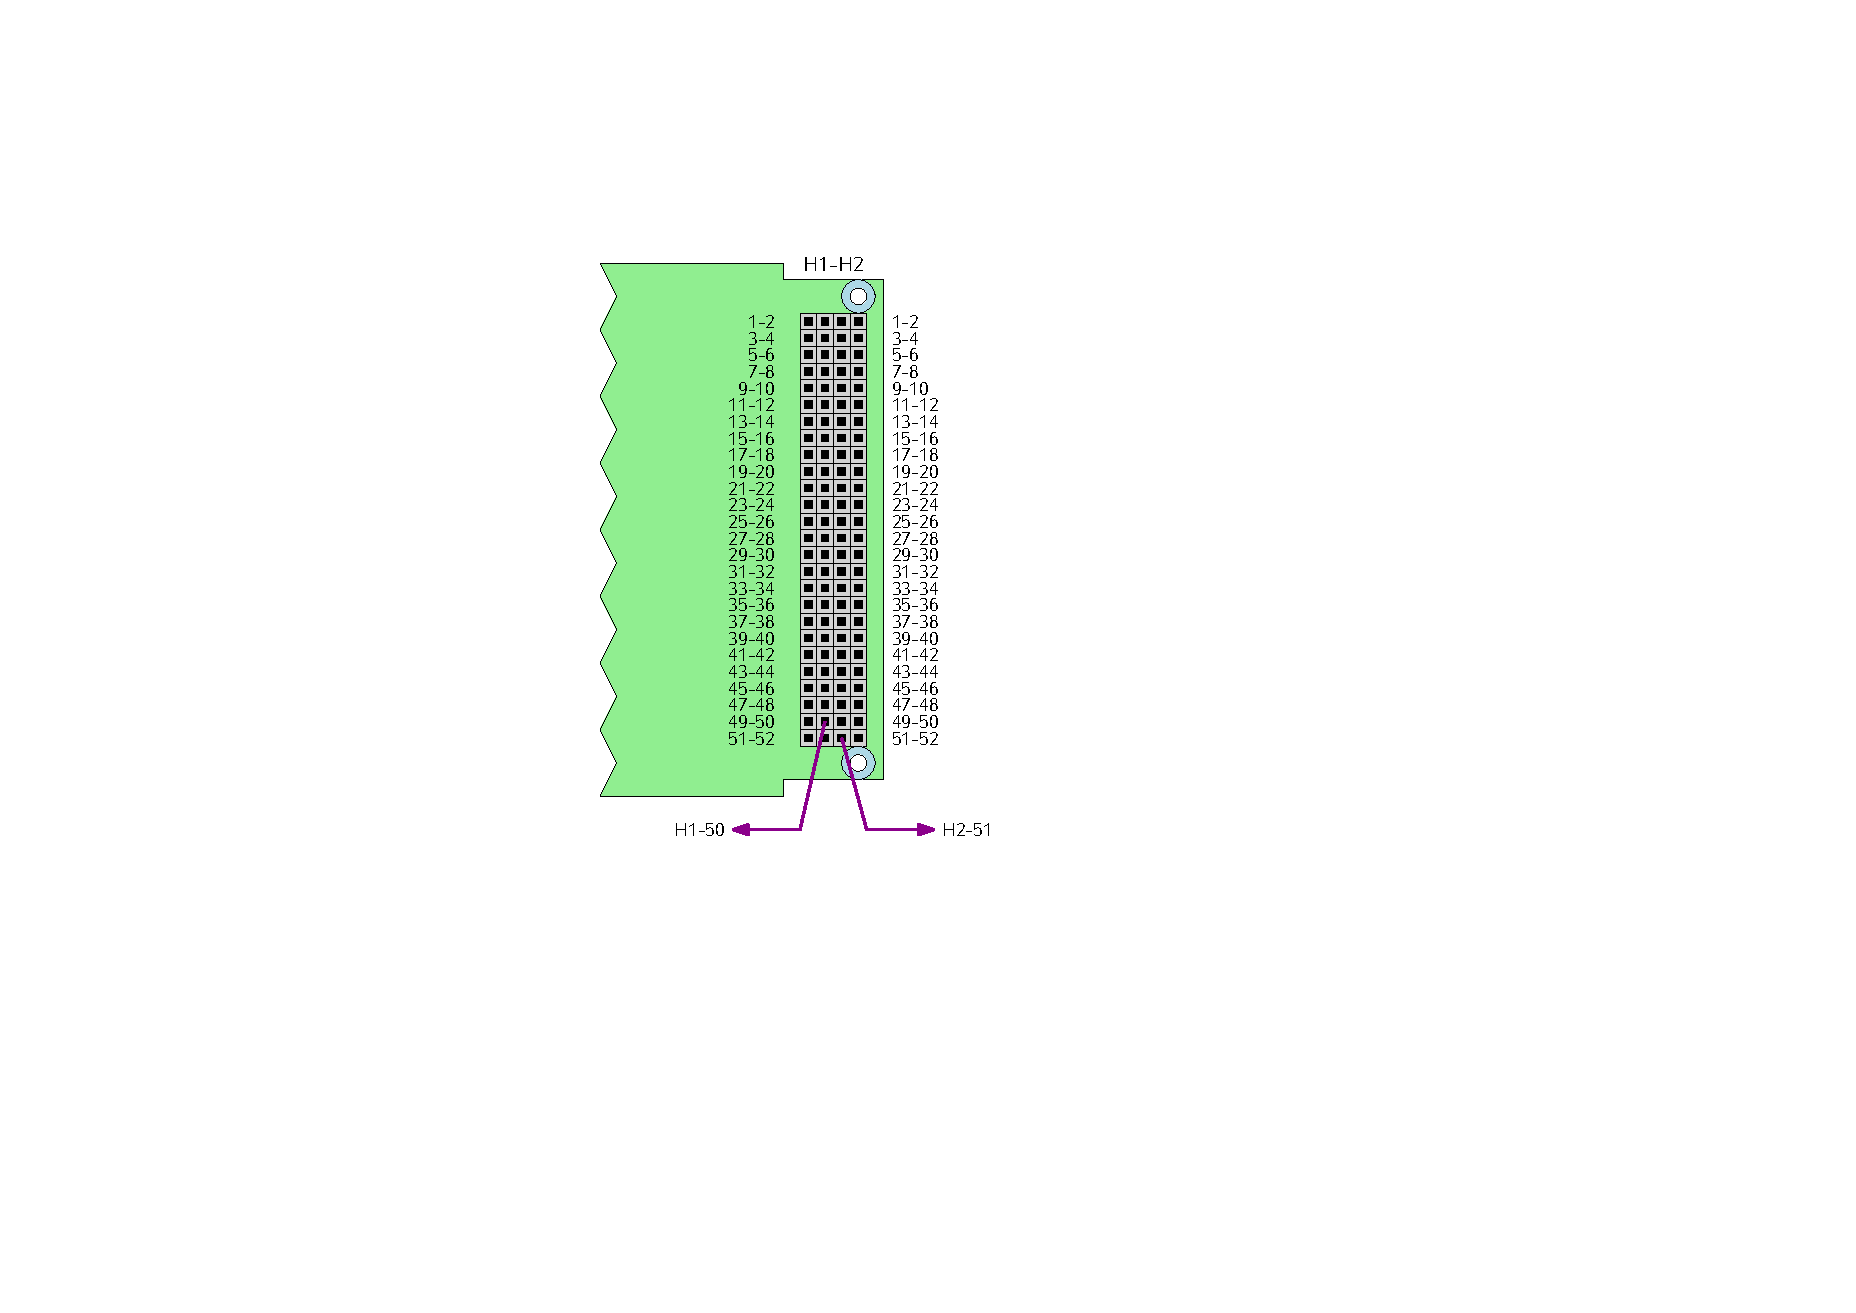
\includegraphics[width=0.5\textwidth]{figures/pc104-diagram}
        \caption{Reference diagram of the PC-104 bus (top view of a generic module).}
        \label{fig:pc104-ref-diagram}
    \end{center}
\end{figure}

\begin{table}[!h]
    \centering
    \begin{tabular}{cllll}
        \toprule[1.5pt]
        \textbf{Pin Row}   & \textbf{H1 Odd}  & \textbf{H1 Even} & \textbf{H2 Odd}  & \textbf{H2 Even} \\
        \midrule
        1-2                & -                & -                & -                & -                \\
        3-4                & -                & -                & -                & -                \\
        5-6                & -                & -                & RA\_1\_UART\_RX  & -                \\
        7-8                & GPIO\_6          & GPIO\_7          & RA\_1\_UART\_TX  & GPIO\_0          \\
        9-10               & RA\_1\_SPI\_INT  & RA\_1\_EN        & -                & -                \\
        11-12              & RA\_0\_SPI\_INT  & RA\_0\_EN        & RA\_1\_SPI\_MOSI & RA\_1\_SPI\_CLK  \\
        13-14              & -                & -                & RA\_1\_SPI\_CS   & RA\_1\_SPI\_MISO \\
        15-16              & -                & -                & -                & -                \\
        17-18              & -                & -                & -                & GPIO\_1          \\
        19-20              & -                & GPIO\_2          & -                & GPIO\_3          \\
        21-22              & -                & -                & -                & GPIO\_4          \\
        23-24              & -                & -                & -                & -                \\
        25-26              & -                & -                & -                & -                \\
        27-28              & -                & -                & VCC\_3V3         & VCC\_3V3         \\
        29-30              & GND              & GND              & GND              & GND              \\
        31-32              & GND              & GND              & GND              & GND              \\
        33-34              & -                & -                & -                & -                \\
        35-36              & RA\_0\_SPI\_CLK  & -                & VCC\_3V3\_ANT    & VCC\_3V3\_ANT    \\
        37-38              & RA\_0\_SPI\_MISO & -                & -                & -                \\
        39-40              & RA\_0\_SPI\_MOSI & RA\_0\_SPI\_CS   & -                & -                \\
        41-42              & -                & -                & -                & GPIO\_5          \\
        43-44              & -                & -                & -                & -                \\
        45-46              & -                & -                & -                & -                \\
        47-48              & -                & -                & -                & -                \\
        49-50              & VCC\_5V\_RA\_0   & VCC\_5V\_RA\_0   & -                & -                \\
        51-52              & VCC\_6V\_RA\_1   & VCC\_6V\_RA\_1   & -                & -                \\
        \bottomrule[1.5pt]
    \end{tabular}
    \caption{PC-104 bus pinout.}
    \label{tab:pc104-pinout}
\end{table}

\begin{table}[!h]
    \centering
    \begin{tabular}{lL{0.3\textwidth}l}
        \toprule[1.5pt]
        \textbf{Signal}  & \textbf{Pin(s)}                  & \textbf{Description} \\
        \midrule
        GND              & H1-29/30/31/32, H2-29/30/31/32   & Ground reference                      \\
        VCC\_3V3         & H2-27, H2-28                     & TTC power supply (3,3 V)              \\
        VCC\_3V3\_ANT    & H2-35, H2-36                     & Antenna power supply (3,3 V)          \\
        VCC\_5V\_RA\_0   & H1-49, H1-50                     & Radio 0 power supply (5 V)            \\
        VCC\_6V\_RA\_1   & H1-51, H1-52                     & Radio 1 power supply (6 V)            \\
        RA\_0\_SPI\_CLK  & H1-35                            & CLK signal of the radio 0 SPI bus     \\
        RA\_0\_SPI\_MISO & H1-37                            & MISO signal of the radio 0 SPI bus    \\
        RA\_0\_SPI\_MOSI & H1-39                            & MOSI signal of the radio 0 SPI bus    \\
        RA\_0\_SPI\_CS   & H1-40                            & CS signal of the radio 0 SPI bus      \\
        RA\_0\_SPI\_INT  & H1-11                            & INT signal of the radio 0 SPI bus     \\
        RA\_1\_SPI\_CLK  & H2-12                            & CLK signal of the radio 0 SPI bus     \\
        RA\_1\_SPI\_MISO & H2-14                            & MISO signal of the radio 0 SPI bus    \\
        RA\_1\_SPI\_MOSI & H2-11                            & MOSI signal of the radio 0 SPI bus    \\
        RA\_1\_SPI\_CS   & H1-13                            & CS signal of the radio 0 SPI bus      \\
        RA\_1\_SPI\_INT  & H1-9                             & INT signal of the radio 0 SPI bus     \\
        RA\_1\_UART\_RX  & H2-5                             & RX signal of the radio 1 UART         \\
        RA\_1\_UART\_TX  & H2-7                             & TX signal of the radio 1 UART         \\
        RA\_0\_EN        & H1-11                            & Radio 0 power enable                  \\
        RA\_1\_EN        & H1-9                             & Radio 1 power enable                  \\
        GPIO\_N          & H1-7/8/19, H2-8/18/20/22/42      & GPIO pin (not used)                   \\
        \bottomrule[1.5pt]
    \end{tabular}
    \caption{PC-104 bus signal description.}
    \label{tab:pc104-signals}
\end{table}

The distribution pattern of pins adopted in this project is a mix of multiple different patterns from CubeSat modules manufacturers, like GomSpace, ISIS and Endurosat. Some pins are positioned to attend specific project requirements, and it is possible that the adopted pattern is not totally compatible to some commercial modules.

\section{Other Electrical Interface}

The module also contains electrical interface through pin headers and picoblades that are used to flash and debug the microcontrollers (CN5, CN3, CN4, CN6), serial communication for status report (CN7, CN8). The C9 connector is used to switch the TTC 2.0 power supply to the MSP-FET. The CN1 and CN2 are directly connected with the antenna I$^{2}$C bus and Y0, Y1 are MCX connectors for the antennas with RF interface with the radios.

\begin{table}[!htb]
    \centering
    \label{tab:icd}
    \begin{tabular}{lccl}
        \toprule[1.5pt]
        \textbf{Connector} & \textbf{Interface} & \textbf{Type} & \textbf{Pins} \\
        \midrule
        \multirow{6}{*}{CN1} & \multirow{6}{*}{I$^{2}$C} & \multirow{6}{*}{PicoBlade} & 3V3 \\
                             &                           &                            & 3V3 \\
                             &                           &                            & I2C\_SDA \\
                             &                           &                            & I2C\_SCL \\
                             &                           &                            & GND \\
                             &                           &                            & GND \\
        \midrule
        \multirow{6}{*}{CN2} & \multirow{6}{*}{I$^{2}$C} & \multirow{6}{*}{PicoBlade} & 3V3 \\
                             &                           &                            & 3V3 \\
                             &                           &                            & I2C\_SDA \\
                             &                           &                            & I2C\_SCL \\
                             &                           &                            & GND \\
                             &                           &                            & GND \\
        \midrule
        \multirow{6}{*}{CN5} & \multirow{6}{*}{JTAG} & \multirow{6}{*}{PicoBlade} & 3V3 \\
                             &                       &                            & TDO\_TDI \\
                             &                       &                            & TCK \\
                             &                       &                            & UART\_TX \\
                             &                       &                            & UART\_RX \\
                             &                       &                            & GND \\
        \midrule
        \multirow{6}{*}{CN6} & \multirow{6}{*}{JTAG} & \multirow{6}{*}{PicoBlade} & 3V3 \\
                             &                       &                            & TDO\_TDI \\
                             &                       &                            & TCK \\
                             &                       &                            & UART\_TX \\
                             &                       &                            & UART\_RX \\
                             &                       &                            & GND \\
        \midrule
        \multirow{3}{*}{CN7} & \multirow{3}{*}{UART} & \multirow{3}{*}{PinHeader} & TX \\
                             &                       &                            & RX \\
                             &                       &                            & GND \\
        \midrule
        \multirow{3}{*}{CN8} & \multirow{3}{*}{UART} & \multirow{3}{*}{PicoBlade} & TX \\
                             &                       &                            & RX \\
                             &                       &                            & GND \\
        \midrule
        \multirow{2}{*}{CN9} & \multirow{2}{*}{Jumper} & \multirow{2}{*}{Pin Header} & 3V3 \\
                             &                         &                      & - \\
        \bottomrule[1.5pt]
    \end{tabular}
    \label{tab:other-elect_interf}
\end{table}

\begin{table}[!htb]
    \centering
    \label{tab:icd}
    \begin{tabular}{lccl}
        \toprule[1.5pt]
        \textbf{Connector} & \textbf{Interface} & \textbf{Type} & \textbf{Pins} \\
        \multirow{14}{*}{CN3} & \multirow{14}{*}{JTAG} & \multirow{14}{*}{Pin Header} & TDO\_TDI \\
                              &                        &                              & 3V3 \\
                              &                        &                              & None \\
                              &                        &                              & None \\
                              &                        &                              & None \\
                              &                        &                              & None \\
                              &                        &                              & TCK \\
                              &                        &                              & None \\
                              &                        &                              & GND \\
                              &                        &                              & None \\
                              &                        &                              & None \\
                              &                        &                              & UART\_TX \\
                              &                        &                              & None \\
                              &                        &                              & UART\_RX \\
        \midrule
        \multirow{14}{*}{CN4} & \multirow{14}{*}{JTAG} & \multirow{14}{*}{Pin Header} & TDO\_TDI \\
                              &                        &                              & 3V3 \\
                              &                        &                              & None \\
                              &                        &                              & None \\
                              &                        &                              & None \\
                              &                        &                              & None \\
                              &                        &                              & TCK \\
                              &                        &                              & None \\
                              &                        &                              & GND \\
                              &                        &                              & None \\
                              &                        &                              & None \\
                              &                        &                              & UART\_TX \\
                              &                        &                              & None \\
                              &                        &                              & UART\_RX \\
        \midrule
        \multirow{2}{*}{Y0} & \multirow{2}{*}{RF} & \multirow{2}{*}{MCX} & RF\_SIGNAL \\
                            &                     &                      & RF\_GND \\
        \midrule
        \multirow{2}{*}{Y1} & \multirow{2}{*}{RF} & \multirow{2}{*}{MCX} & RF\_SIGNAL \\
                            &                     &                      & RF\_GND \\
        \bottomrule[1.5pt]
    \end{tabular}
    \caption{Other electrical interfaces.}
    \label{tab:other-elect_interf}
\end{table}

\section{PCB}

\subsection{Dimensions}

The TTC PCB Dimensions follows the industry standarts for Cubesats defined by ISIS and GOMSPACE with $89,15 mm$ by $92,13 mm$. See \cite{nasa-handout}.  The outline is specific to improve the physic integration between the modules and payloads.

\begin{figure}[!ht]
    \begin{center}
        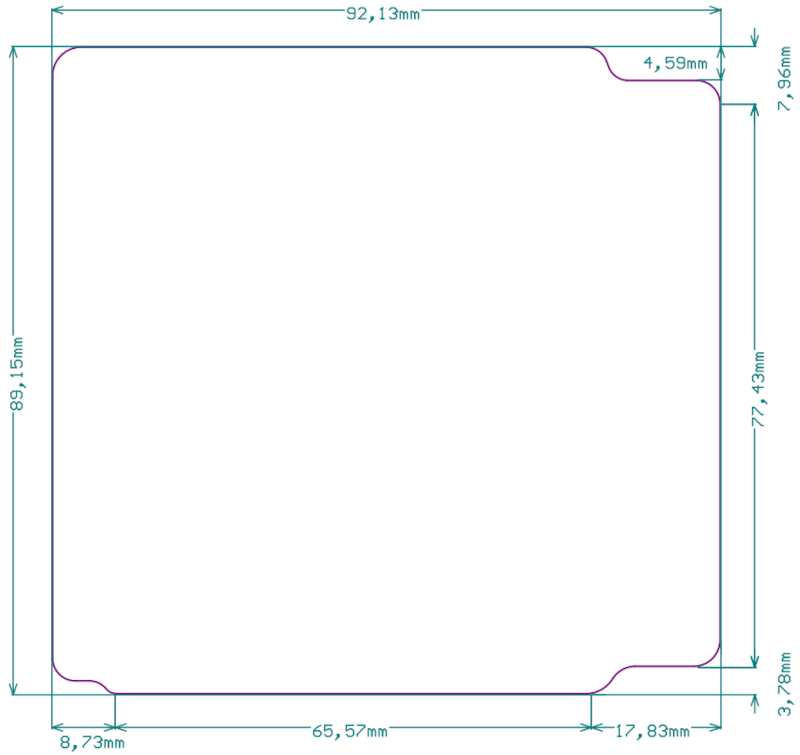
\includegraphics[width=0.6\textwidth]{figures/board-dimensions.png}
        \caption{Board dimensions for the TTC 2.0 module.}
        \label{fig:product-tree}
    \end{center}
\end{figure}

\subsection{PCB Layout}

The TTC 2.0 module contains only two layers: the top and bottom of the PCB. See \autoref{fig:ttc2-pcb-top} and \autoref{fig:ttc2-pcb-bottom}. The PCB Flight Model will have the following manufacturing specifications:

\begin{itemize}
    \item PCB specs.: IPC 6012 Class 3
    \item PCB thickness: 1,6 mm
    \item Material: TG170 FR-4
    \item Surface finish: ENIG
    \item Board finish: Conformal coating application
\end{itemize}

\begin{figure}[!ht]
    \begin{center}
        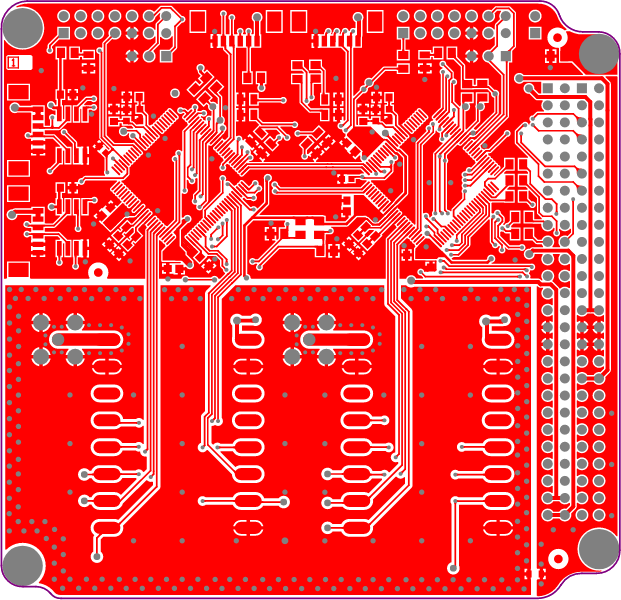
\includegraphics[width=0.7\textwidth]{figures/ttc2-layout-top.png}
        \caption{Top layer of the TTC 2.0 layout.}
        \label{fig:ttc2-layout-top}
    \end{center}
\end{figure}

\begin{figure}[!ht]
    \begin{center}
        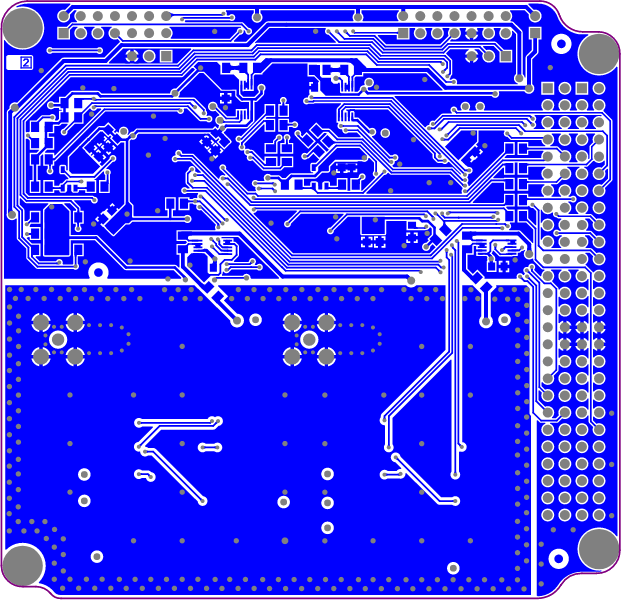
\includegraphics[width=0.7\textwidth]{figures/ttc2-layout-bottom.png}
        \caption{Bottom layer of the TTC 2.0 layout.}
        \label{fig:ttc2-layout-bottom}
    \end{center}
\end{figure}

\subsection{Board Peripherals}

The TTC 2.0 counts with external (to the microcontroller) current sensors, watchdog and radio.

\subsubsection{Power Sensor}

The power sensor (INA226AQDGSRQ1) uses an I$^{2}$C interface to communicate with the microcontroller. There is four of this sensor in the module, one for each microcontroller and one for each radio module. It monitors voltage and power from a given bus and also voltage, power and current from a shunt resistor ($0.1$ $\Omega$). The final measurement is continuous and made by an average of 128 measurements with an interval of 588 $\mu$s between.

\subsubsection{External Watchdog}

Besides the internal watchdog of the microcontroller, there is also a redundant external one. For that, the IC TPS3823 is used. It has a voltage monitor and an watchdog timer, with a timeout of 1600 ms.

\subsubsection{Radio Module}

The Radio (NiceRF RF4463F30) uses an SPI interface with the microcontroller. The radio has special alimentation of 5V from the EPS module to be able to have 30 dBm of output power. The radio is half-duplex, has integrated power amplifier and RF switches since it uses a single antenna.

\begin{figure}[!ht]
    \begin{center}
        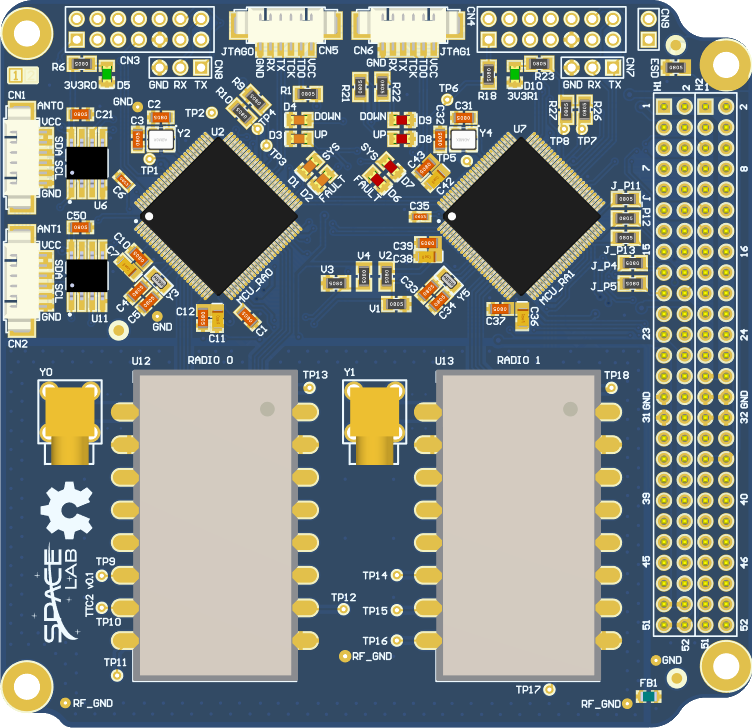
\includegraphics[width=0.7\textwidth]{figures/ttc2_pcb_top.png}
        \caption{Upper surface of the TTC 2.0 PCB.}
        \label{fig:ttc2-pcb-top}
    \end{center}
\end{figure}

\begin{figure}[!ht]
    \begin{center}
        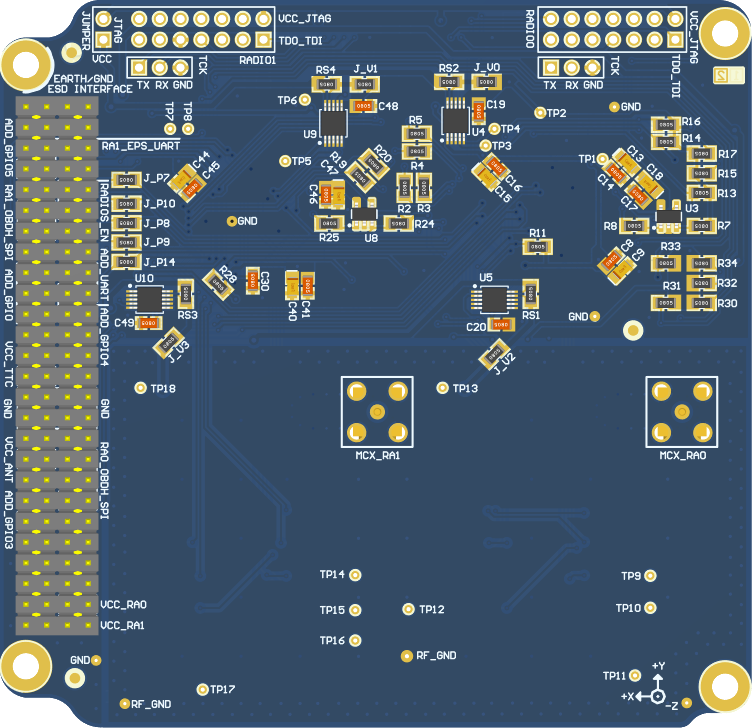
\includegraphics[width=0.7\textwidth]{figures/ttc2_pcb_bottom.png}
        \caption{Lower surface of the TTC 2.0 PCB.}
        \label{fig:ttc2-pcb-bottom}
    \end{center}
\end{figure}
